\section{\K 双极型晶体三极管}
\Par 双极型晶体管(bipolar junction transistorBJT),又称三极管,它是组成各种电子电路的核心器件.三极管一般可以分为PNP型和NPN型两种三极管.如图\ref{fig:三极管结构}所示,三极管的三个部分分别被称作发射区(E)、基区(B)和集电区(C),同时,在三个区的两两交界处,形成两个PN结,分别称为发射结和集电结.为了使三极管能有电流放大作用,在制造时使其发射区杂质浓度很高、基区很薄且杂质浓度很低.我们主要讨论NPN型三极管及其电路.

\begin{figure}[htbp]
	\centering
	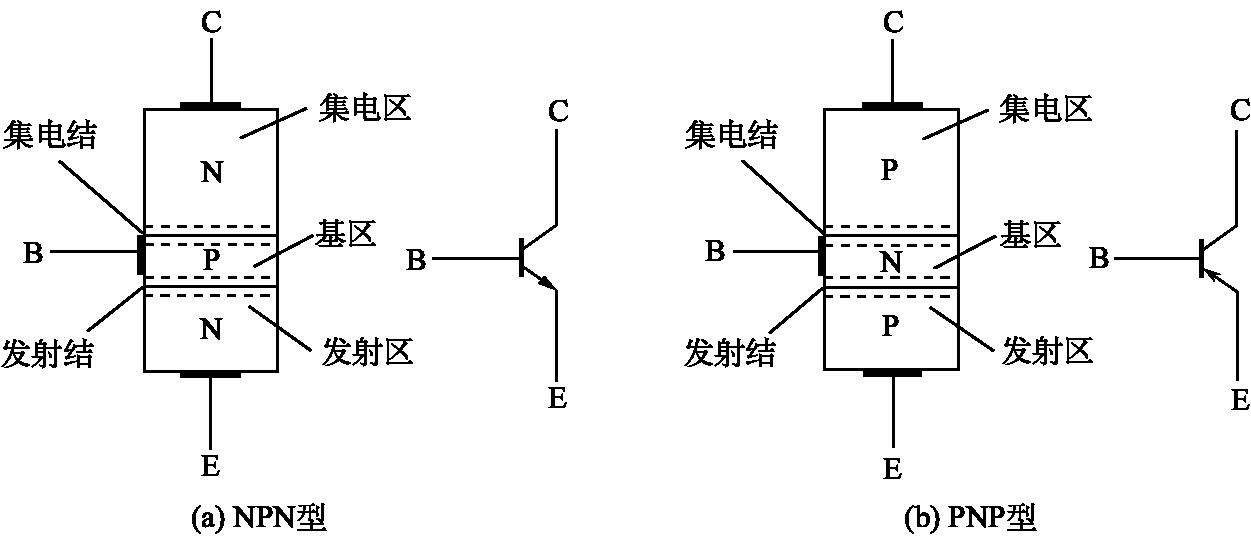
\includegraphics[width=0.65\textwidth]{三极管结构.jpg}
	\caption{三极管结构}
	\label{fig:三极管结构}
\end{figure}

